\documentclass[11pt,ngerman]{article}
\usepackage{geometry}
\usepackage[T1]{fontenc}
\usepackage[utf8]{inputenc}
\usepackage{babel}
\usepackage{hyperref}
\usepackage{lmodern}%get scalable font
\usepackage{titling}
\usepackage{relsize}
\usepackage{biblatex}
\usepackage{glossaries}
\usepackage{paralist}
\usepackage[table, dvipsnames]{xcolor}
\usepackage{booktabs}
\usepackage{tabularx}
\usepackage{float}
\restylefloat{table}
\usepackage{setspace}
\usepackage{multicol}
\usepackage{graphicx}
\usepackage[most]{tcolorbox}
\usepackage{enumitem}
\usepackage{textcomp}

% Link colors
\hypersetup{
    colorlinks,
    linkcolor={blue},
    citecolor={red},
    urlcolor={blue}
}

\usepackage{lipsum} % generates lorem ipsum => remove again when finished

\geometry{a4paper, top=25mm, left=25mm, right=25mm, bottom=20mm,
    headsep=10mm, footskip=12mm}

% Glossary
% Das Glossar definiert alle wichtigen Begriffe zur Sicherstellung einer einheitlichen Terminologie.
% Es sollen keine allgemeinen Begriffe erklärt werden, die den Adressaten bekannt sind (z. B. Java, CPU etc.).
% Glossareinträge müssen im Text verwendet werden damit diese im Glossar im Appendix \printglossary angezeigt werden
\makeglossaries
\loadglsentries{glossary} % loads glossary definitions from external file

\pretitle{\begin{center}\linespread{1.5}\huge}
    \posttitle{\par\end{center}\vspace{0.5em}}

% double quotes macro
% usage: \quotes{arg1}  => in text: "arg1"
\newcommand{\quotes}[1]{``#1''}

\begin{document}

    \title{Tron Licht-Motorräder Computerspiel\\
        \vspace{1cm}
        Lösungsarchitektur \\
        \vspace{0.5cm}
        \small{}ZHAW  School of Engineering
        \vspace{1.5cm}
    }
    \author{
        Akca, Deniz\\
        \small{akcaden1@students.zhaw.ch}
        \and
        Holenstein, Christian\\
        \small{holenchr@students.zhaw.ch}
        \and
        Huber, Patrick\\
        \small{huberpa4@students.zhaw.ch}
        \and
        Iten, Mike\\
        \small{itenmik1@students.zhaw.ch}
        \vspace{1.5cm}
    }
   \date{\today}

    \maketitle
    \newpage

    \tableofcontents
    \listoftables
    \listoffigures
    \newpage

    % First section
    \section{Anwendungsfälle}
        Anwendungsfälle Übersicht:
        \begin{multicols}{2}
            \begin{itemize}
               \item  \hyperref[ssec:UC1Lobbyerstellen]{UC1: Lobby erstellen - \quotes{fully dressed}}
                \item\hyperref[ssec:UC2Spielspielen]{UC2: Spiel spielen - \quotes{fully dressed}}
                \item \hyperref[sssec:UC3EinAusloggen]{UC3: Ein \& Ausloggen  - \quotes{casual}}
                \item \hyperref[sssec:UC4Lobbybeitreten]{UC4: Lobby beitreten - \quotes{casual}}
                \item \hyperref[sssec:UC5Registrieren]{UC5: Registrieren - \quotes{brief}}
                \item \hyperref[sssec:UC6Passwortsetzen]{UC6: Passwort zurücksetzen - \quotes{brief}}
                \item  \hyperref[sssec:UC7Freundeeinladen]{UC7: Freunde einladen - \quotes{brief}}
                \item \hyperref[sssec:UC8Statistikenbetrachten]{UC8: Statistiken betrachten - \quotes{brief}}
           \end{itemize}
        \end{multicols}

        \subsection{Anwendungsfalldiagramm}
            \begin{figure}[H]
                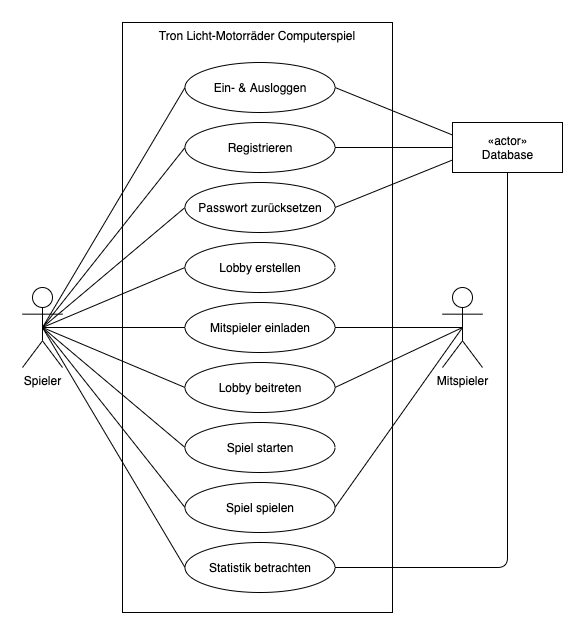
\includegraphics[scale=0.77]{figures/Use-case-modell.png}
                \caption{Anwendungsfalldiagramm - Tron Licht-Motorräder Computerspiel}
            \end{figure}

        \subsection{Hauptanwendungsfälle}
            Wir haben zwei Hauptanwendungsfälle identifiziert:
             \begin{itemize}
                \item  \hyperref[ssec:UC1Lobbyerstellen]{UC1: Lobby erstellen - \quotes{fully dressed}}
                \item\hyperref[ssec:UC2Spielspielen]{UC2: Spiel spielen - \quotes{fully dressed}}
            \end{itemize}
            Die Hauptanwendungsfälle werden in den nächsten zwei Abschnitten detailliert ausgeführt.

            \subsubsection{UC1: Lobby erstellen - \quotes{fully dressed}}
            \label{ssec:UC1Lobbyerstellen}
                \begin{tcolorbox}[enhanced, breakable, sharp corners, width=\dimexpr\textwidth-15mm\relax ,enlarge left by=10mm ,fontupper=\linespread{1.1}\selectfont, boxrule=1pt, title={UC1: Lobby erstellen}, colback=white, colframe=gray!22, coltitle=black]

                    \textbf{Anwendungsfall:} Lobby erstellen \\
                    \textbf{Ebene:} Anwenderziel \\
                    \textbf{Primärakteur:} Spieler \\
                    \textbf{Stakeholder und Interessen:}
                    \begin{itemize}
                        \item \textit{Spieler}: Möchte mit anderen Spielern zusammen in einer \Gls{Lobby} beitreten oder seine eigene \Gls{Lobby} erstellen. Kann die Rolle des Lobby-Erstellers haben.
                        \item \textit{Mitspieler}: Möchten mit anderen Spielern zusammen in einer \Gls{Lobby} beitreten. Kann die Rolle des Lobby-Erstellers haben.
                        \item \textit{Lobby-Ersteller}:  Möchte das Spiel starten, wenn alle Spieler bereit sind.
                        \item \textit{System}: Möchte mehrere Spieler in einer \Gls{Lobby} haben, um ein Spiel starten zu können.
                    \end{itemize}
                    \textbf{Vorbedingungen:} Alle Spieler sind entweder mit einem persönlichen oder Gastkonto angemeldet.\\
                    \textbf{Nachbedingungen:} Mehrere Spieler oder auch einzelne Spieler befinden sich in \Glspl{Lobby}. Das System ist in der Lage in den \Glspl{Lobby} mit mehreren Spielern ein Spielgang zu starten. \\
                    \\  \textbf{Standardablauf:}
                    \begin{enumerate}
                        \item Spieler/Mitspieler wechselt zur Lobbyansicht der Anwendung.
                        \item Spieler/Mitspieler wählt eine bestehende öffentliche \Gls{Lobby} aus.
                        \item Spieler/Mitspieler tritt diese \Gls{Lobby} bei.
                        \item Spieler und Mitspieler warten in \Gls{Lobby} auf weitere Mitspieler..
                        \item Spieler/Mitspieler klicken auf \quotes{Bereit}
                        \item Lobby-Ersteller startet das Spiel.
                        \item System überprüft ob alle Spieler in der \Gls{Lobby} bereit sind.
                    \end{enumerate}
                    \textit{Falls nicht alle Spieler bereit sind, muss der Lobby-Ersteller zu einem weiteren Zeitpunkt nochmals Schritt 6 ausführen. Erst wenn alle Spieler bereit sind, wird mit Schritt 8 fortgefahren.}
                    \begin{enumerate}[resume]
                        \item System startet das Spiel.
                    \end{enumerate}
                    \textit{Es ist nun nicht mehr möglich - als Spieler oder Mitspieler - dieser \Gls{Lobby} beizutreten.} \\
                    \textit{Spiel wird gespielt …, Ende des Spiels.}
                    \begin{enumerate}[resume]
                        \item System öffnet \Gls{Lobby} wieder
                    \end{enumerate}
                    \textit{Spieler/Mitspieler können \Gls{Lobby} beitreten. Punkt 3 bis 9 wiederholen sich, bis Spieler sich entscheidet, das Spiel oder die \Gls{Lobby} zu verlassen.} \\
                    \\ \textbf{Erweiterungen (oder alternative Abläufe):}
                    \begin{itemize}
                        \item[2a.] Spieler können eigene \Gls{Lobby} erstellen:
                        \begin{enumerate}
                            \item Spieler klickt auf \Gls{Lobby} erstellen.
                            \item Spieler wählt ob die \Gls{Lobby} öffentlich zugänglich (public) ist oder nur für Freunde (private).
                            \item System erstellt eine \Gls{Lobby}.
                            \item System fügt den Spieler als Lobby-Ersteller der \Gls{Lobby} hinzu.
                        \end{enumerate}
                        \item[2b.] Spieler können privaten \Glspl{Lobby} von Freunden über einen Link beitreten:
                        \begin{enumerate}
                            \item Spieler öffnet Einladung.
                            \item Spieler öffnet den Link im Browser.
                            \item System fügt Spieler der \Gls{Lobby} des Freundes hinzu.
                        \end{enumerate}
                        \item[4a.] Spieler können \Gls{Lobby} verlassen:
                        \begin{enumerate}
                            \item Spieler/Mitspieler verlassen \Gls{Lobby}
                        \end{enumerate}
                        \item[4b.] Spieler/Mitspieler können weiter in der \Gls{Lobby} bleiben und weiterspielen:
                        \begin{enumerate}
                            \item Spieler/Mitspieler verlassen die \Gls{Lobby} nicht
                        \end{enumerate}
                    \end{itemize}
                    \textbf{Spezielle Anforderungen:}
                    \begin{itemize}
                        \item Sobald ein Mitspieler der \Gls{Lobby} beigetreten ist, läuft ein Timer. Falls der Timer abgelaufen ist und der Mitspieler noch nicht bestätigt hat, wird dieser automatisch abgelehnt.
                        \item Maximale Spieleranzahl muss eingehalten werden. Es gibt eine obere Grenze von Mitspielern, die durch den Spieler definiert wird.
                        \item Internationalisierung der Sprache in den Textanzeigen.
                    \end{itemize}

                \end{tcolorbox}

            \subsubsection{UC2: Spiel spielen - \quotes{fully dressed}}
            \label{ssec:UC2Spielspielen}
                \begin{tcolorbox}[enhanced, breakable, sharp corners, width=\dimexpr\textwidth-15mm\relax ,enlarge left by=10mm ,fontupper=\linespread{1.1}\selectfont, boxrule=1pt, title={UC2: Spiel spielen}, colback=white, colframe=gray!22, coltitle=black]

                    \textbf{Anwendungsfall:} Spiel spielen \\
                    \textbf{Ebene:} Anwenderziel \\
                    \textbf{Primärakteur:} Spieler \\
                    \textbf{Stakeholder und Interessen:}
                    \begin{itemize}
                        \item \textit{Spieler}: Möchte als letzter Spieler übrig bleiben
                        \item \textit{Mitspieler}: Möchte als letzter Spieler übrig bleiben.
                        \item \textit{Lobby-Ersteller}:  Möchte das Spiel starten, wenn alle Spieler bereit sind.
                        \item \textit{System}: Möchte alle Spieler - bereit zum spielen - in einer \Gls{Lobby} haben, um ein Spiel starten zu können.
                    \end{itemize}
                    \textbf{Vorbedingungen:} Mindestens 2 Spieler sind im Spiel.\\
                    \textbf{Nachbedingungen:} Der letzte Spieler im Spiel wurde Sieger. Spiel wurde erfolgreich beendet. \Gls{Lobby} wird erneut angezeigt. \\
                   \\  \textbf{Standardablauf:}
                    \begin{enumerate}
                        \item System lädt Spiel.
                        \item System platziert Spieler/Mitspieler (Spielcharakter) in einem gewissen Abstand zum Spielfeldrand und zu den Mitspielern, jeweils in möglichst entgegengesetzter Richtung, auf dem Spielfeld.
                        \item System zeigt Countdown an. Nach Ablauf des Countdowns beginnt das Spiel.
                        \item System beginnt Startbewegung der Spieler mit konstanter Geschwindigkeit in Richtung Spielfeldmitte.
                    \end{enumerate}
                    \textit{Alle Spieler/Mitspieler auf dem Spielfeld behalten die konstante Geschwindigkeit bei bis zum Ausscheiden oder Ende des Spiels.}
                    \begin{enumerate}[resume]
                        \item System erzeugt Hindernis vom Startpunkt des Spielers/Mitspielers bis zu dessen aktueller Position.
                        \item System übergibt Spieler/Mitspieler die Kontrolle des jeweiligen Spielcharakters.
                    \end{enumerate}
                    \textit{Schritt 4 - 6 folgen ohne Zeitverzögerung aufeinander.}
                    \begin{enumerate}[resume]
                        \item Spieler/Mitspieler können, durch drücken einer Pfeiltaste, die Richtung um jeweils exakt 90\textdegree\ ändern.
                        \item Das durch den Spieler/Mitspieler erzeugte Hindernis, wächst mit der Bewegung und in der jeweiligen Bewegungsrichtung.
                    \end{enumerate}
                    \textit{Das vom Spieler/Mitspieler erzeugte Hindernis, bleibt auf dem Spielfeld bestehen bis zum Ausscheiden oder Sieg des Spielers/Mitspielers, in allen folgenden Schritten.}
                    \begin{enumerate}[resume]
                        \item System koordiniert in kurzen Intervallen alle Bewegungen der Spieler/Mitspieler und überprüft deren Positionen und etwaige Kollisionen.
                    \end{enumerate}
                    \textit{System wiederholt Schritt 7 - 9 bis Kollision erkannt wird.}
                    \begin{enumerate}[resume]
                        \item System entfernt Spieler/Mitspieler mit Kollision vom Spielfeld und zeigt eine entsprechende Meldung an.
                    \end{enumerate}
                    \textit{System wiederholt Schritt 7 - 10 bis ein einziger Spieler/Mitspieler auf dem Spielfeld übrig bleibt.}
                    \begin{enumerate}[resume]
                        \item System zeigt bei letztem Spieler/Mitspieler eine Siegesmeldung an.
                        \item System beendet das Spiel.
                        \item System zeigt die Statistiken des Spiels bei allen Spielern/Mitspielern an.
                        \item System öffnet - nach Ablauf eines Timers  - erneut die \Gls{Lobby}.
                    \end{enumerate}
                    \textbf{Erweiterungen (oder alternative Abläufe):}
                    \begin{itemize}
                        \item[?a.] blah
                            \begin{enumerate}
                                \item blah
                                \item blah
                                \item blah
                            \end{enumerate}
                    \end{itemize}
                    \textbf{Spezielle Anforderungen:}
                     \begin{itemize}
                        \item blah
                    \end{itemize}

                \end{tcolorbox}

            \newpage
            \subsubsection{System-Sequenzdiagramm (SSD)}
                 Das System-Sequenzdiagramm für \quotes{Lobby erstellen} und \quotes{Spiel spielen}:
                 \begin{figure}[H]
                     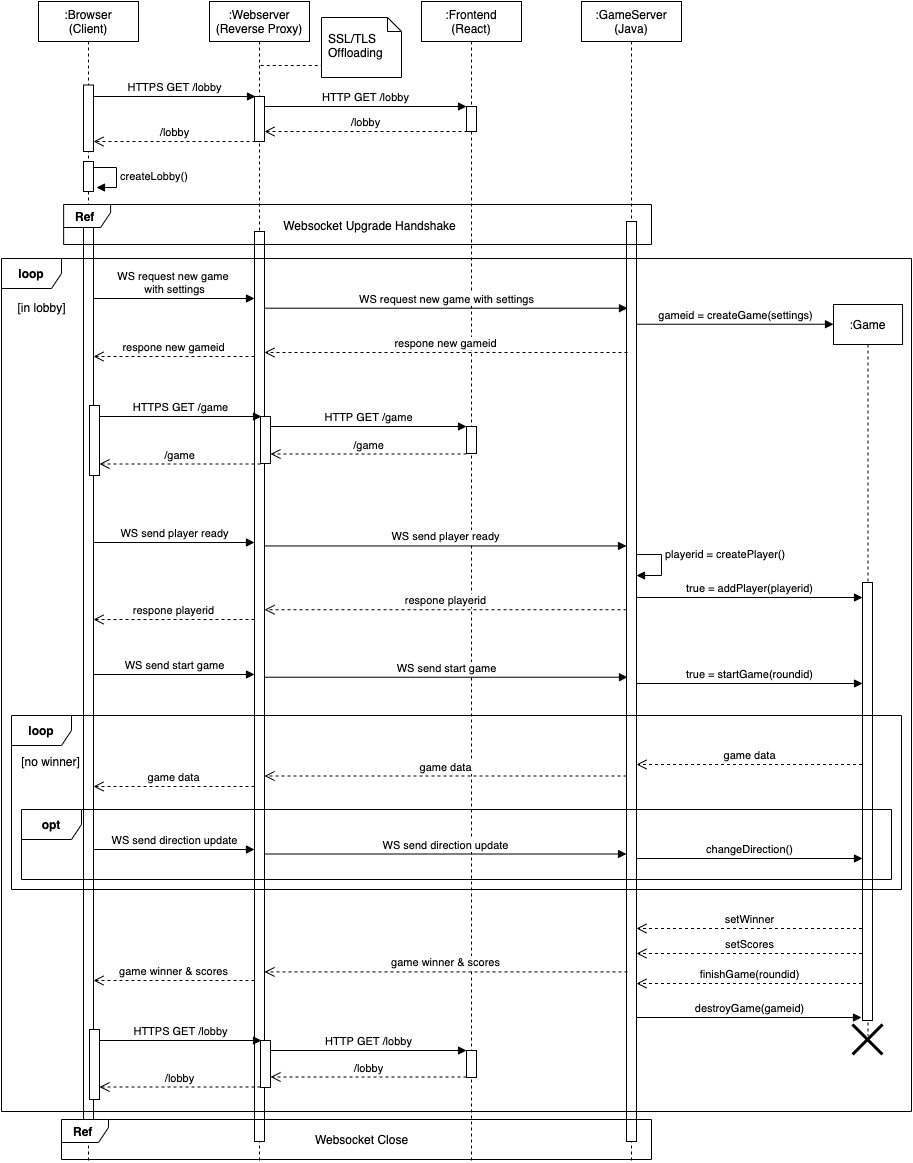
\includegraphics[scale=0.5]{figures/SystemSequenceDiagram.png}
                     \caption{System-Sequenzdiagramm - \quotes{Lobby erstellen} \&  \quotes{Spiel spielen}}
                 \end{figure}
                 \newpage
                \noindent \textbf{Referenz: \Gls{Websocket} Upgrade Handshake} \\
                \autoref{fig:SSDReferenzWebsocketUpgrade} zeigt den Upgrade Request der HTTP(S) Verbindung  zu \Gls{Websocket}.
                \begin{figure}[H]
                    \centering
                    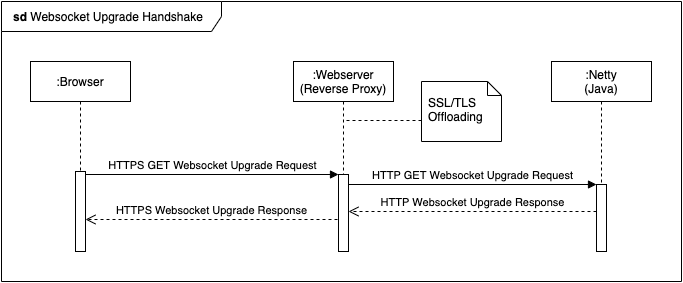
\includegraphics[scale=0.6]{figures/SSD-Websocket_Upgrade_Handshake.png}
                    \caption{SSD Referenz - \Gls{Websocket} Upgrade Handshake}
                    \label{fig:SSDReferenzWebsocketUpgrade}
                \end{figure}
                \noindent \textbf{Referenz: \Gls{Websocket} Close} \\
                \autoref{fig:SSDReferenzWebsocketClose} zeigt das schliessen der \Gls{Websocket}-Verbindung.
                \begin{figure}[H]
                    \centering
                    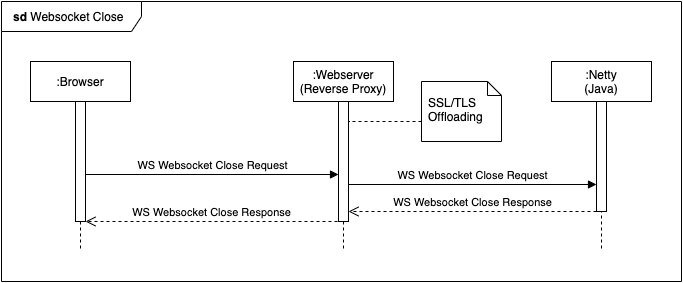
\includegraphics[scale=0.6]{figures/SSD-Websocket_Close.png}
                    \caption{SSD Referenz - \Gls{Websocket} Close}
                    \label{fig:SSDReferenzWebsocketClose}
                \end{figure}

        \subsection{Übrige Anwendungsfälle}
            \subsubsection{UC3: Ein \& Ausloggen  - \quotes{casual}}
            \label{sssec:UC3EinAusloggen}
                \begin{tcolorbox}[enhanced, breakable, sharp corners, width=\dimexpr\textwidth-15mm\relax ,enlarge left by=10mm ,fontupper=\linespread{1.1}\selectfont, boxrule=1pt, title={UC3: Ein \& Ausloggen }, colback=white, colframe=gray!22, coltitle=black]
                     \textit{Standardszenario:} Der Spieler navigiert sich zum Login-Bereich der Anwendung. Der Spieler gibt die korrekten Eingabedaten seines Kontos ein. Die Anwendung überprüft die Eingabedaten und meldet den Spieler an. Der
Spieler ist nun in der Anwendung mit seinem persönlichen Konto angemeldet.\newline
                     \newline
                     \textit{Alternative Szenarios:} \newline
                     Der Spieler gibt die falschen Eingabedaten für ein Konto ein. Das System weist den Spieler
daraufhin, dass die Eingabedaten falsch sind und schlägt dem Spieler vor noch einmal die  Eingabedaten einzugeben. \newline
                     \newline
                     Der Spieler möchte sich aus dem System ausloggen. Der Spieler navigiert sich in der Anwendung auf
sein Profil und wählt die Funktion «Logout» aus. Das System beendet die Session und der Spieler
wird zum Login-Screen weitergeleitet.
                \end{tcolorbox}

             \subsubsection{UC4: Lobby beitreten - \quotes{casual}}
             \label{sssec:UC4Lobbybeitreten}
                 \begin{tcolorbox}[enhanced, breakable, sharp corners, width=\dimexpr\textwidth-15mm\relax ,enlarge left by=10mm ,fontupper=\linespread{1.1}\selectfont, boxrule=1pt, title={UC4: Lobby beitreten }, colback=white, colframe=gray!22, coltitle=black]
                     \textit{Standardszenario:} Der Spieler navigiert auf der Startseite zu dem Lobbybereich, dort kann der Spieler einer öffentlichen Lobby beitreten. \newline
                     Nun befindet sich der Spieler in einer Lobby mit anderen Spielern.\newline
                     \newline
                     \textit{Alternative Szenarios:} \newline
                     Der Spieler erhält einen Link eines Freundes. Mit dem Link kann der Spieler einer privaten Lobby eines Freundes beitreten. \newline
                     Der Spieler befindet sich nun in derselben Lobby mit einem Freund.
                 \end{tcolorbox}

             \subsubsection{UC5: Registrieren - \quotes{brief}}
             \label{sssec:UC5Registrieren}
                 \begin{tcolorbox}[enhanced, breakable, sharp corners, width=\dimexpr\textwidth-15mm\relax ,enlarge left by=10mm ,fontupper=\linespread{1.1}\selectfont, boxrule=1pt, title={UC5: Registrieren}, colback=white, colframe=gray!22, coltitle=black]
                     Der Spieler navigiert sich zum Registrier-Bereich der Anwendung. Der Spieler gibt seinen Usernamen, Passwort und E-Mail an.\newline
                     Die Anwendung überprüft ob der Username bereits belegt ist. Der Spieler besitzt nun ein eigenes Konto
                 \end{tcolorbox}

             \subsubsection{UC6: Passwort zurücksetzen - \quotes{brief}}
             \label{sssec:UC6Passwortsetzen}
                \begin{tcolorbox}[enhanced, breakable, sharp corners, width=\dimexpr\textwidth-15mm\relax ,enlarge left by=10mm ,fontupper=\linespread{1.1}\selectfont, boxrule=1pt, title={UC6: Passwort zurücksetzen}, colback=white, colframe=gray!22, coltitle=black]
                    Der Spieler navigiert sich zum Login-Bereich der Anwendung. Dort hat der Spieler die Möglichkeit sein Passwort zurück zu setzen.\newline
                    Nun kann der Spieler ein neues Passwort angeben.
                \end{tcolorbox}

             \subsubsection{UC7: Freunde einladen - \quotes{brief}}
             \label{sssec:UC7Freundeeinladen}
                \begin{tcolorbox}[enhanced, breakable, sharp corners, width=\dimexpr\textwidth-15mm\relax ,enlarge left by=10mm ,fontupper=\linespread{1.1}\selectfont, boxrule=1pt, title={UC7: Freunde einladen}, colback=white, colframe=gray!22, coltitle=black]
                    Der Spieler erstellt eine private Lobby. Der Spieler erhält ein Link, mit welchem Freunde beitreten können.\newline
                    Die beigetretenen Freunde befinden sich nun mit dem Spieler in derselben Lobby.
                \end{tcolorbox}

             \subsubsection{UC8: Statistiken betrachten - \quotes{brief}}
             \label{sssec:UC8Statistikenbetrachten}
                \begin{tcolorbox}[enhanced, breakable, sharp corners, width=\dimexpr\textwidth-15mm\relax ,enlarge left by=10mm ,fontupper=\linespread{1.1}\selectfont, boxrule=1pt, title={UC8: Statistiken betrachten}, colback=white, colframe=gray!22, coltitle=black]
                    Der Spieler navigiert auf der Startseite der Anwendung zu den Statistiken. Dort ist eine Liste einsehbar in welcher alle Spieler mit ihren Punkten einsehbar sind.
                \end{tcolorbox}

    \section{Zusätzliche Anforderungen}

    \subsection{Funktionalität}

    \subsection{Benutzbarkeit}

    \subsection{Zuverlässigkeit}

    \subsection{Effizienz}

    \subsection{Änderbarkeit (Wartbarkeit)}

    \subsection{Internationalisierung}

    \subsection{Einschränkungen}

    \subsubsection{Designeinschränkungen}

    \subsubsection{Implementierungseinschränkungen}

    \subsubsection{Schnittstelleneinschränkungen}

    \section{Domänenmodell}

    \section{Softwarearchitektur}

    \section{Design-Artefakte}

    \section{Implementation}

    \section{Projektmanagement}


    % Appendix after this
     \newpage

    \section{Appendix}
    \textit{Hinweis: Glossar-Referenznummern sind Seitennummern}
    \printglossary

\end{document}

